\section{Grundlagen Halbleiterphysik}

\subsection{Bohrsches Atommodell}

\myul{\textbf{1. Bohrsches Postulat:}}\\
        Es gibt nur bestimmte diskrete Schalen, die für ein Elektron erlaubt sind.\\
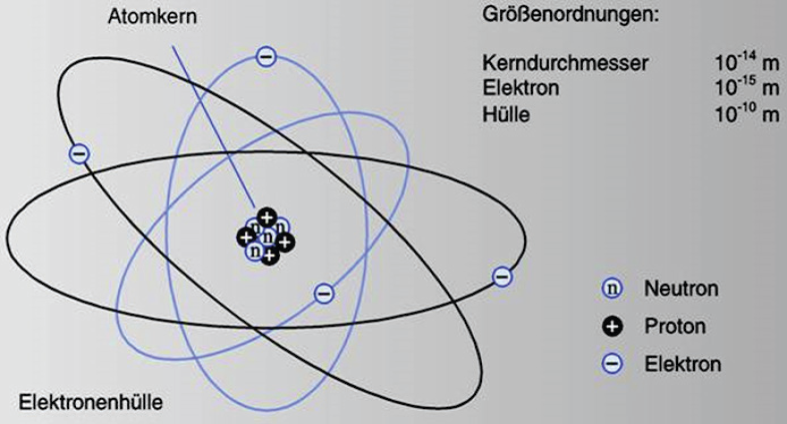
\includegraphics[width=0.95\linewidth]{images/V02_01.png}

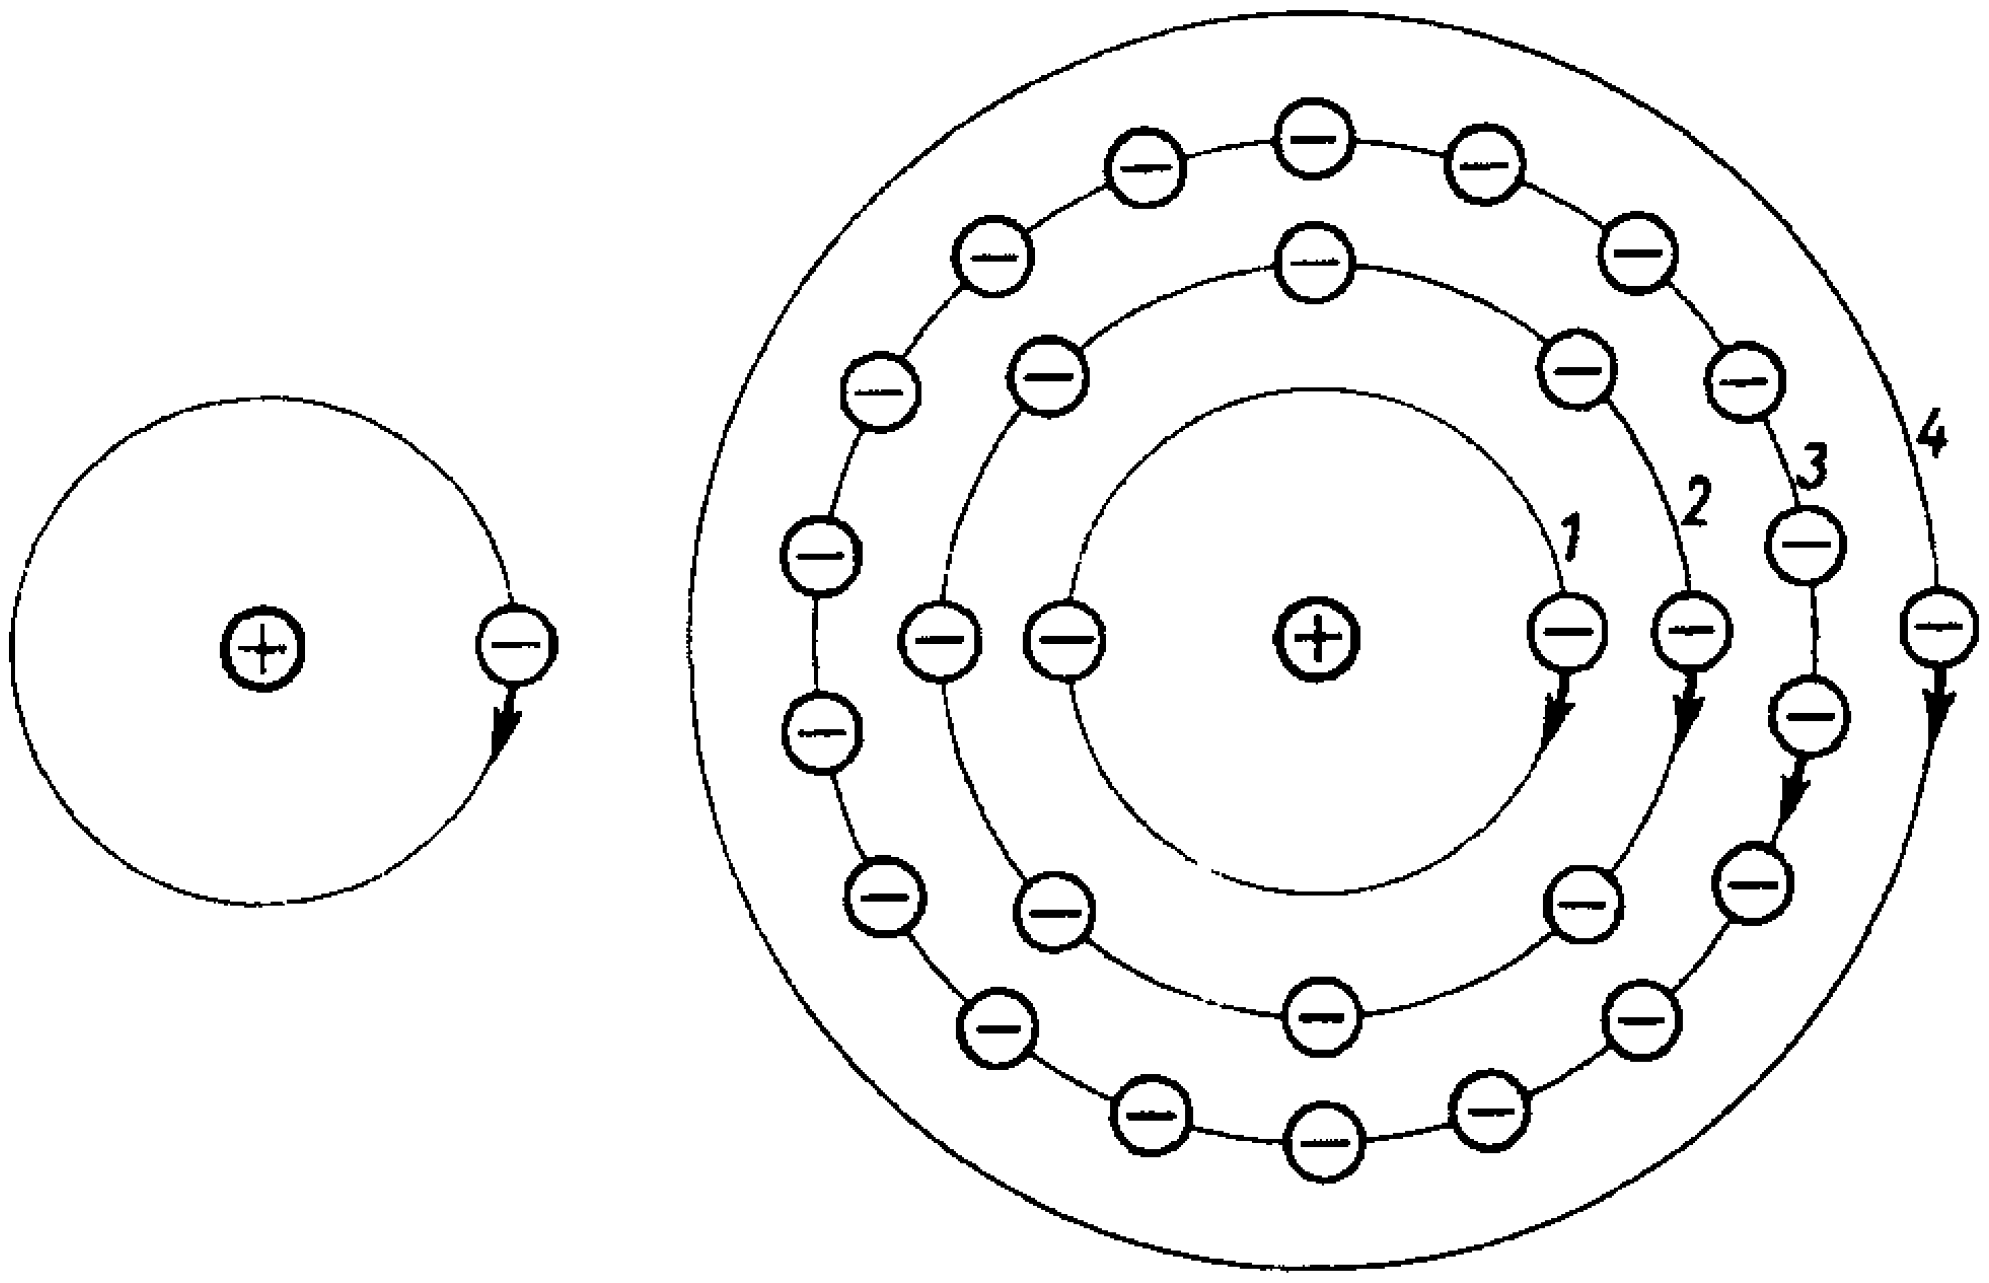
\includegraphics[width=0.75\linewidth]{images/V02_02.png}

Links: Wasserstoff\\
Rechts: Kupfer\\


\renewcommand{\arraystretch}{1.5}
    \begin{tabular}{|l|c|c|}
        \hline
        \textbf{Elementarteilchen} & \textbf{Ruhemasse} & \textbf{Ladung} \\
        \hline
        Proton & $1{,}673 \cdot 10^{-27} \, \text{kg}$ & $+e$ \\
        Neutron & $1{,}675 \cdot 10^{-27} \, \text{kg}$ & $0$ \\
        Elektron & $0{,}911 \cdot 10^{-30} \, \text{kg}$ & $-e$ \\
        \hline
    \end{tabular}

Elementarladung $e = 1.602 \cdot 10^{-19} C$\\



\myul{\textbf{2. Bohrsches Postulat}}\\
Der übergang eines Elektrons von einer Schale zur anderen erfolgt unter Emission der Absorption von elektromagnetischer Strahlung.\\

\begin{minipage}[t]{0.48\columnwidth}
    \textbf{Emission}\\
    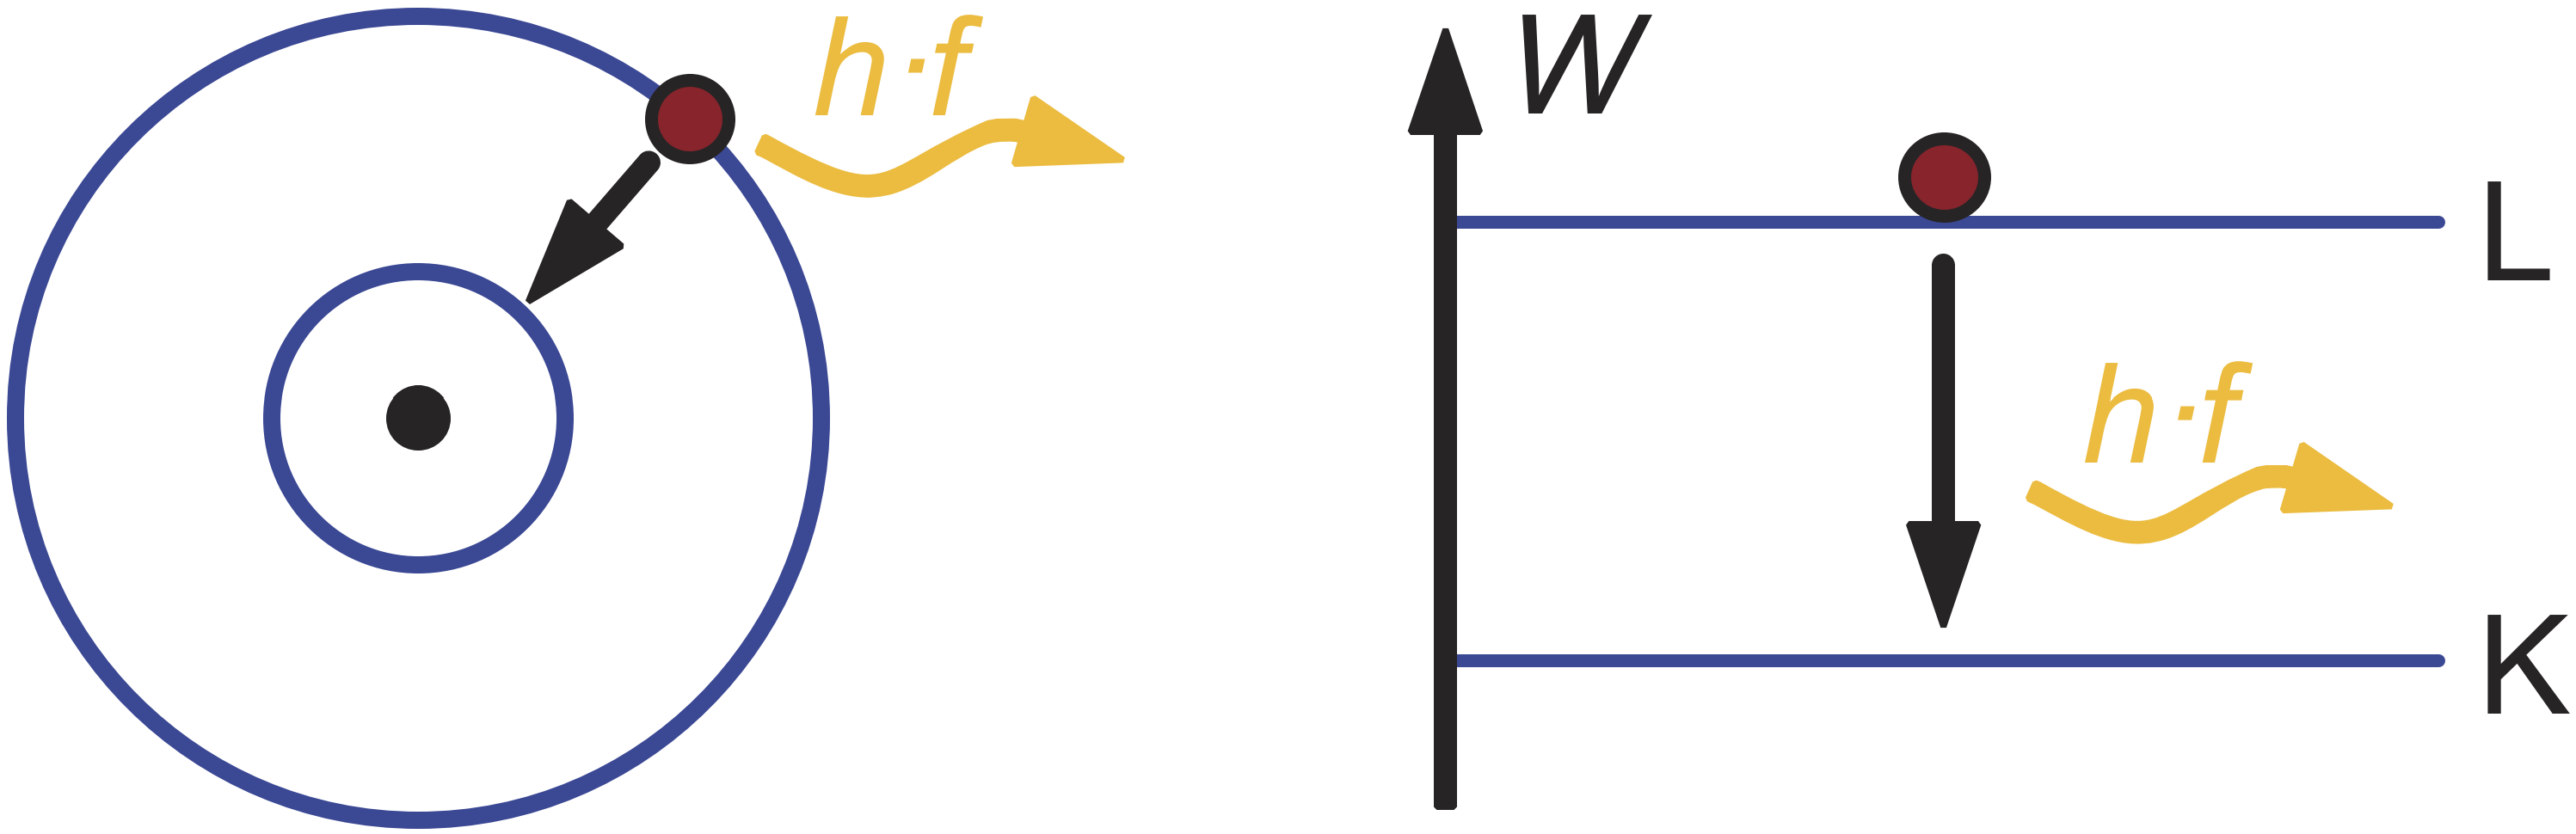
\includegraphics[width=0.85\linewidth]{images/V02_03.png}
\end{minipage}
\hfill
\begin{minipage}[t]{0.48\columnwidth}
    \textbf{Absorption}\\
    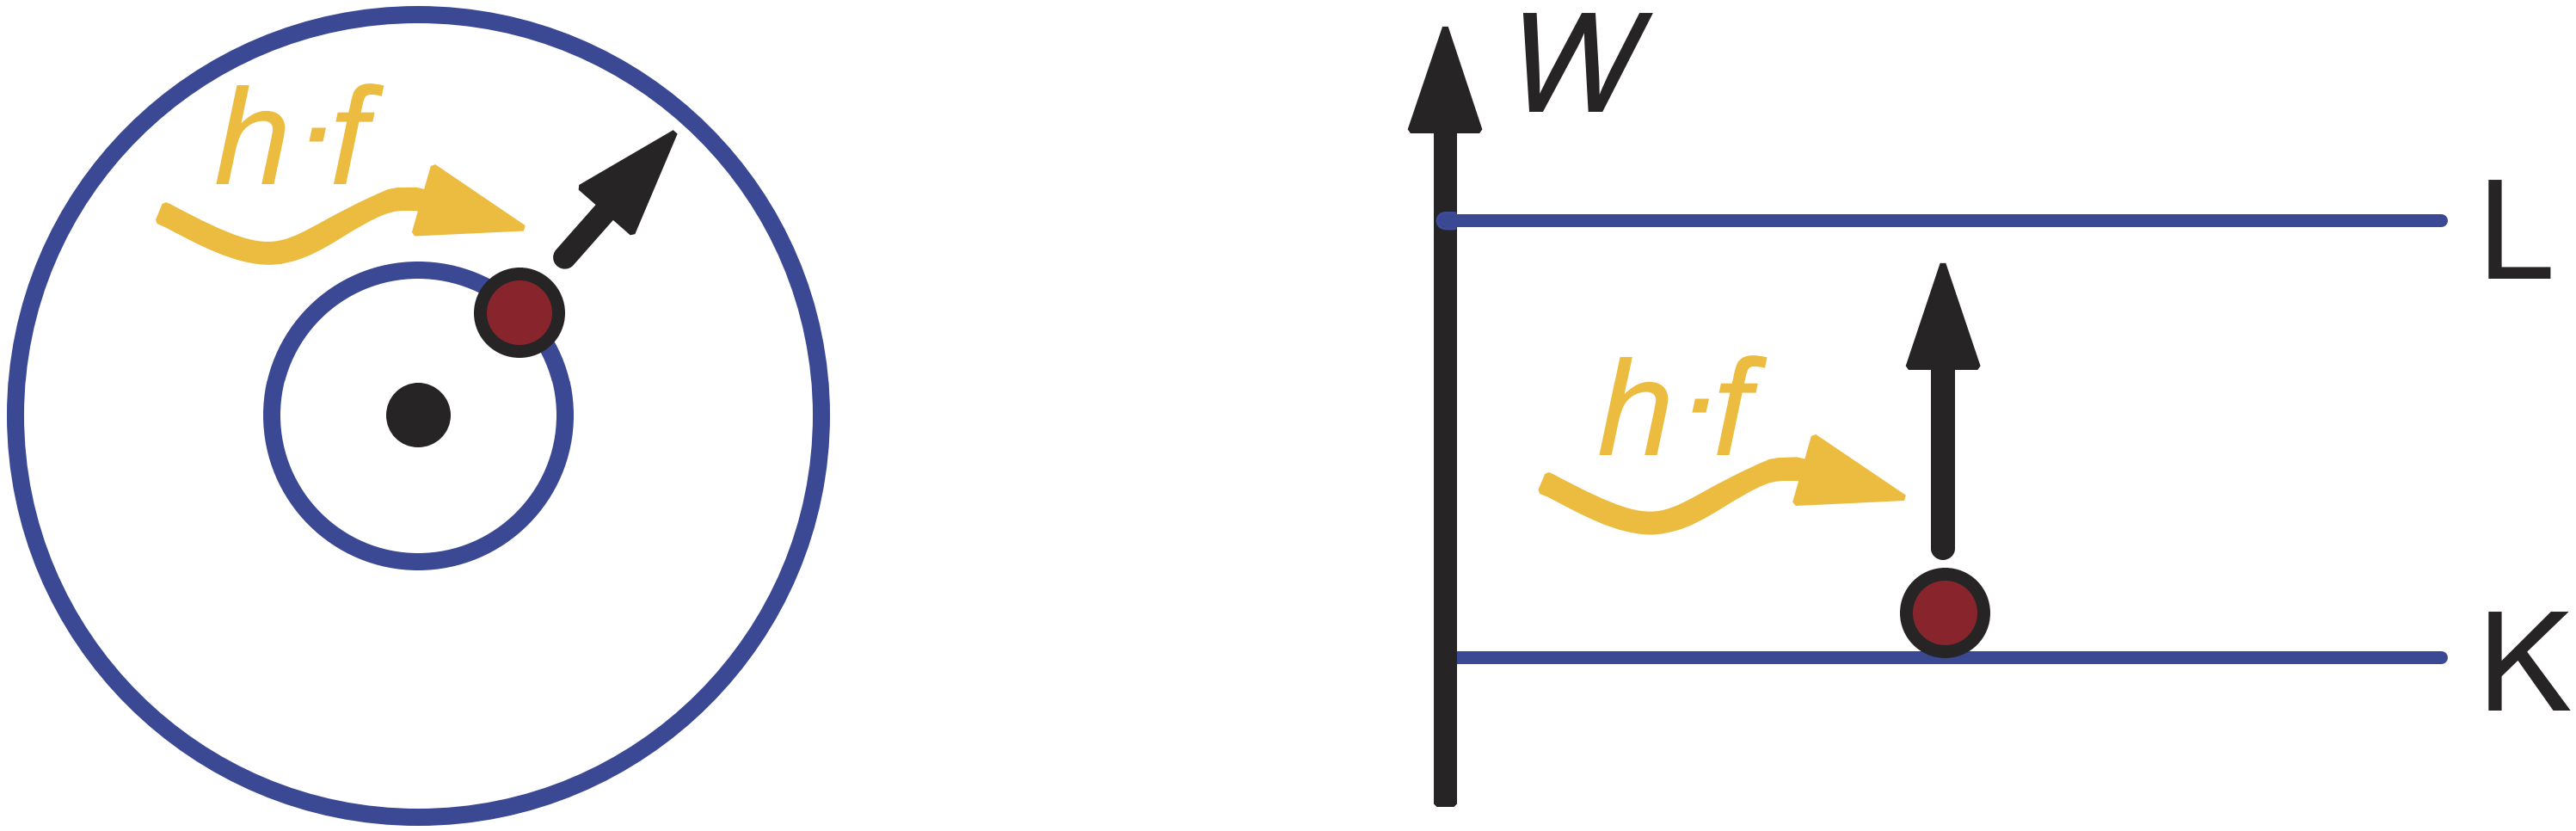
\includegraphics[width=0.85\linewidth]{images/V02_04.png}
\end{minipage}

\vspace{0.5cm}

$\boxed{\Delta W = \lvert W_2 - W_1 \rvert = h \cdot f}$ \quad $\boxed{\lambda = \frac{c_0}{f}}$ \quad $c_0 \approx 3 \cdot 10^8 \frac{m}{s}$

\renewcommand{\arraystretch}{1.2} % Erhöht Zeilenhöhe für bessere Lesbarkeit
\begin{tabular}{@{} l p {4cm} l @{}}
    $[\Delta W]$    & Energiedifferenz          \dotfill & $Ws$ \\
    $[W_1]$         & Energie vor dem Übergang  \dotfill & $Ws$ \\
    $[W_2]$         & Energie nach dem Übergang \dotfill & $Ws$ \\
    $[h]$           & Plancksches Wirkungsquantum \dotfill & $Ws^2$ \\
    $[f]$           & Frequenz \dotfill & $\frac{1}{s}$ \\
    $[c_0]$         & Lichtgeschwindigkeit \dotfill & $\frac{m}{s}$ \\
    $[\Lambda]$     & Wellenlänge \dotfill & $m$ \\
\end{tabular}































